% !TeX program = xelatex
% !TeX encoding = UTF-8
\documentclass{JXUSTmodeling}
\usepackage{float}
\usepackage{subcaption}
\sisetup{
	inter-unit-product = \ensuremath{{}\cdot{}}
}
\biaoti{}
\keyword{}
\begin{document}
\begin{abstract}

\end{abstract}
\section{问题背景与重述}
\label{sec:1}
\subsection{问题背景}
\label{sub:1.1}
运载火箭从地面起飞到进入预定轨道，需要在有限推进剂条件下同时完成高度提升、水平加速和轨道圆化。飞行过程中，中心引力、大气阻力、地球自转、质量持续下降和级间分离共同改变火箭状态；滑行时长与二子级推力方向还会影响重力损失和推进剂利用率。因此，建立统一的分阶段动力学模型并对末级控制进行优化，是评价入轨能力和设计节能轨迹的基础。
\subsection{问题重述}
\label{sub:1.2}
某两级液体运载火箭从赤道发射场起飞，目标是将10\si{t}有效载荷送入高度400\si{km}的近地圆轨道。飞行过程依次包括一子级垂直上升与程序转弯、一二子级分离后的无动力滑行以及二子级点火入轨。题目给定两级质量、推进剂、推力、比冲及气动参数，要求建立动力学模型并完成四项任务：复现基准控制下的全程轨迹；调整滑行时间和二子级线性俯仰程序实现圆轨道入轨；进一步优化滑行时间和俯仰角程序以减少二子级耗油；在二子级可于60\%～100\%额定推力间连续节流时重新求解最省油控制策略。
\section{问题分析}
\label{sec:2}
\subsection{问题一分析}
\label{sub:2.1}
问题一的控制律和各阶段持续条件均已给定，核心是构造能够统一描述推力、中心引力、旋转大气阻力和变质量效应的分阶段动力学系统。连续飞行由常微分方程刻画，一子级燃尽与二子级燃尽由推进剂耗尽事件定位，级间分离则表现为质量的瞬时跃变。

考虑到起飞瞬间速度为零，直接把速度大小和飞行路径角作为独立状态会出现路径角初值不稳定的问题，因此采用径向速度与切向速度作为基本状态，再由二者计算速度和路径角。求解结果除给出四条状态曲线外，还需检查一、二子级燃尽时刻、分离质量跃变以及终端状态是否满足目标圆轨道条件。
\subsection{问题二分析}
\label{sub:2.3}
问题二保留问题一的一子级轨迹，把滑行时间、二子级俯仰角变化率和二子级工作时间作为未知量。目标圆轨道提供高度、径向速度和切向速度三项独立条件，因此可建立三元非线性打靶方程，并通过多初值求根检验解的稳定性与唯一性。

三个待定参数对终端状态的影响具有明显耦合：滑行时间改变点火高度和速度方向，俯仰角变化率决定推力在径向与切向上的分配，工作时间控制总速度增量和耗油量。求解时需要对三项终端残差进行尺度归一化，并排除工作时间超过燃尽极限或剩余推进剂为负的非物理解。
\subsection{问题三分析}
\label{sub:2.4}
问题三中的二子级推力恒定，推进剂质量流率为常数，最小耗油量与最短工作时间等价。俯仰角程序属于连续函数，采用控制参数化把推力—速度夹角离散为有限节点，在每个候选控制下正向积分状态方程，并用圆轨道终端条件约束非线性规划。网格加密用于检验控制离散误差。

该问题的决策对象由三个标量参数扩展为一条连续控制函数，属于有限时间燃料最优控制问题。将推力方向写成速度方向与相对夹角之和，可以直接施加夹角边界，并避免分别限制俯仰角和路径角。节点数增加会提高控制自由度，同时也扩大非线性规划规模，因此采用由粗到细的网格和热启动策略。
\subsection{问题四分析}
\label{sub:2.5}
问题四增加节流比后，质量流率不再恒定，不能继续以工作时间直接衡量燃料。应以节流比的时间积分构造燃料目标，并同步优化夹角和节流节点。由于扩大控制集合并不必然严格改善目标值，需要通过多初值、网格加密和独立高精度复算判断节流是否真正产生省油收益。

节流降低会减小单位时间耗油率，但也会延长有动力飞行并增加重力作用时间，因此最优节流不应仅凭直观指定。模型必须允许节流节点在60\%～100\%区间自由变化，再由终端圆轨道约束和燃料目标共同决定其取值；最后还应将问题四与问题三在相同节点数下比较，以区分节流收益与离散误差。
\section{模型的假设}\label{sec:3}
模型假设主要包括：
\begin{enumerate}
	\item 地球为均匀球体，重力采用中心引力模型，火箭在赤道平面内运动。
	\item 火箭视为变质量质点，忽略姿态动力学、结构振动、推力建立过程及级间分离冲量。
	\item 一子级采用题给指数大气密度和常阻力系数；大气随地球刚性旋转，二子级阶段忽略气动阻力。
	\item 发动机比冲与额定推力在各自工作阶段保持不变，关机前不考虑二次点火。
	\item 问题三、四中，二子级推力—速度夹角满足$\abs{\alpha} \leqslant 15^\circ$，作为控制可实现性的附加约束；不另设角速度与节流变化率约束。
	\item 400 km圆轨道以终端高度400 km、径向速度为0和切向速度等于当地圆轨道速度表征。
\end{enumerate}

\section{符号说明}\label{sec:4}
\subsection{常量声明}
本题目求解过程中，使用到的常量定义如\ref{tab:constant_table}所示。
\begin{table}[htbp]
	\centering
	\caption{常量说明}
	\label{tab:constant_table}
	\renewcommand{\arraystretch}{0.9}
	\begin{tabularx}{\textwidth}{cccX}
		\toprule
		符号 & 常量值 & 单位 & \multicolumn{1}{c}{含义}\\
		\midrule
		$R_E$
		& $6.371\times10^{6}$
		& \si{\metre}
		& 地球半径 \\
		$\Omega_E$
		& $7.292115\times10^{-5}$
		& \si{\radian\per\second}
		& 地球自转角速度 \\ 
		$\mu$
		& $3.986004418\times10^{14}$
		& \si{\metre\cubed\per\second\squared}
		& 地球引力参数 \\
		$g_0$
		& $9.80665$
		& \si{\metre\per\second\squared}
		& 标准重力加速度 \\
		
		$I_{\mathrm{sp} i}$
		& 题目给定
		& \si{\second}
		& 第$i$级发动机比冲 \\
		
		$F_{\max i}$
		& 题目给定
		& \si{\newton}
		& 第$i$级发动机额定最大推力 \\
		\bottomrule
	\end{tabularx}
\end{table}
\subsection{变量声明}
本题目求解过程中，使用到的主要变量及其符号定义见\ref{tab:variable_table}。
\begin{table}[H]
	\centering
	\caption{变量说明}\label{tab:variable_table}
	\renewcommand{\arraystretch}{0.9}
	\begin{tabularx}{\textwidth}{YYX}
	\toprule
	符号 & 单位 & \multicolumn{1}{c}{含义} \\
	\midrule
	$r$ & \si{\metre} & 地心距 \\ 
	$h$ & \si{\metre} & 火箭高度 \\
	$v_t$ & \si{\metre\per\second} & 切向速度 \\
	$v_r$ & \si{\metre\per\second} & 径向速度 \\
	$\theta$ & \si{\radian} & 惯性极角 \\
	$\gamma$ & \si{\radian}
	& 飞行路径角 \\
	
	$\psi$
	& \si{\radian}
	& 推力俯仰角 \\
	$m$
	& \si{\kilogram}
	& 火箭总质量 \\
	
	$T$
	& \si{\newton}
	& 发动机推力 \\
	
	$u$
	& 无量纲
	& 二子级节流比 \\
	
	$D_r$
	& \si{\newton}
	& 阻力的径向分量 \\
	
	$D_t$
	& \si{\newton}
	& 阻力的切向分量 \\
	
	$\rho$
	& \si{\kilogram\per\metre\cubed}
	& 大气密度 \\
	
	$\tau$
	& \si{\second}
	& 滑行时间 \\
	
	$t_{c2}$
	& \si{\second}
	& 二子级工作时间 \\
	
	$k_2$
	& \si{\degree\per\second}
	& 二子级俯仰角变化率 \\
	
	$q$
	& \si{\second}
	& 等效满推力时间 \\
	\bottomrule
	\end{tabularx}
\end{table}
\section{模型的建立与求解}
\label{sec:5}
\subsection{问题一模型建立及求解}
\label{sec:5.1}
\subsubsection{状态变量与环境模型}
在地心惯性极坐标系内选取状态向量$\mathbf{x}=\left[r, \theta ,v_r, v_t, m\right]^\mathrm{T}$。速度大小与飞行路径角分别为：
\begin{equation}
	\begin{aligned}
		v &= \sqrt{v_r^2 + v_t^2}, \\
		\gamma &= \operatorname{atan2}(v_r, v_t).
	\end{aligned}
	\label{eq:1}
\end{equation}

赤道发射点在惯性系中具有向东切向速度，则初始状态可写为：
\begin{equation}
	\mathbf{x}=\left[R_E, 0, 0, v_0, M_0 \right]^{\mathrm{T}}
	\label{eq:2}
\end{equation}
其中，$v_0 = \Omega_E R_E$。

采用径向—切向速度状态后，起飞时无需人为指定飞行路径角；当速度从零逐渐增大时，可由$\operatorname{atan2}(v_r,v_t)$连续恢复路径角。火箭在当地基底上的矢量受力关系为
\begin{equation}
	m \dot{\mathbf{v}}=T\left(
	\mathrm{sin}\psi \mathbf{e}_r
	+
	\mathrm{cos} \psi \mathbf{e}_t
	\right)
	+
	D_r\mathbf{e}_r
	+
	D_t\mathbf{e}_t
	-
	\frac{\mu m}{r^2}\mathbf{e}_r
	\label{eq:base}
\end{equation}

大气相对速度的切向分量为$v_{rel, t}=v_t - \Omega_Er$，径向分量仍为$v_r$。由题给指数密度模型得到一子级阻力分量：
\begin{equation}
	\begin{aligned}
		V_{rel} 
		&=
		\sqrt{v_r^2  + v_{rel, t}^2},\\
		\rho(h)
		&=
		\rho_0 e^{-\frac{h}{h_0}}, \\
		D_r
		&=
		-\frac{1}{2}\rho C_D S V_{\mathrm{rel}}v_r, \\
		D_t
		&=
		-\frac{1}{2}\rho C_D S V_{\mathrm{rel}}
		\left(v_t-\Omega_E r\right).
	\end{aligned}
	\label{eq:4}
\end{equation}
其中$S = 12.5$为题目给定的一子级飞行气动阻力参考面积，$C_D = 0.3$为阻力系数。
\subsubsection{分阶段变质量动力学}
推力俯仰角$\psi$以当地水平面为零方向。将推力、阻力与中心引力分别投影到径向和切向，可得统一动力学方程。
\begin{equation}
	\left\{
	\begin{aligned}
		\dot{r}
		&=
		v_r\\
		\dot{\theta}
		&=
		v_t / r, \\
		\dot{v_r}
		&=
		v_t^2 / r - \mu / r^2 + (T sin\psi + D_r ) / m, \\
		\dot{v_t} 
		&= 
		-v_r v_t/r + (Tcos \psi + D_t)/m, \\
		\dot{m}
 		&=
		- T / (I_{sp} g_0).
	\end{aligned}
	\right.
\end{equation}
其中$v_t^2 / r$与$-v_r v_t/r$来自极坐标基底随位置转动产生的几何项。飞行阶段运载火箭的质量变化由发动机消耗燃料产生。当发动机关闭时，$T=0$，运载火箭质量不再发生变化。

一子级仅在前10\si{s}保持$\psi_1=90^\circ$，此后按$0.4^\circ/ s$线性减小。燃尽条件为$m=M_0 - m_{p 1}$。随后瞬时抛离40\si{t}结构质量。滑行阶段取$T=0$且忽略阻力；60\si{s}后二子级全推力点火并令$\psi_2= \gamma$，直至将燃料消耗完毕。由题意可列出运载火箭飞行阶段的判定函数：
\begin{equation}
	\left\{
	\begin{aligned}
		g_1(\mathbf{x})
		&=
		m - (M_0 -m_{p 1})\\
		g_2(\mathbf{x})
		&=
		m - (m_{s 2} + m_payload).
	\end{aligned}
	\right.
\end{equation}
其中事件$g_1(\mathbf{x})=0$时，一子级推进剂耗尽、发动机关机，同理事件$g_2(\mathbf{x})=0$表示二子级耗尽推进剂。位置和速度在分离瞬间连续，仅质量发生跃变，因而整个模型属于连续动力学与离散事件组合的混杂系统。各飞行阶段运载火箭的受力、速度与推力方向关系如\ref{fig:1}所示。
\begin{figure}[htbp]
	\centering
	\begin{subfigure}[b]{0.45\textwidth}
	\centering
	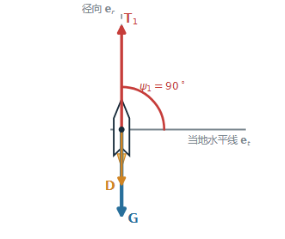
\includegraphics[width=\linewidth]{figure/1-1.png}
	\caption{垂直上升阶段}
	\label{fig:1-1}
	\end{subfigure}
	\hfill
	\begin{subfigure}[b]{0.45\textwidth}
		\centering
		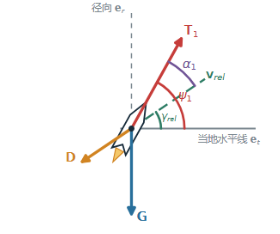
\includegraphics[width=\linewidth]{figure/1-2.png}
		\caption{一子级动力飞机阶段}
		\label{fig:1-2}
	\end{subfigure}
	\begin{subfigure}[b]{0.45\textwidth}
		\centering
		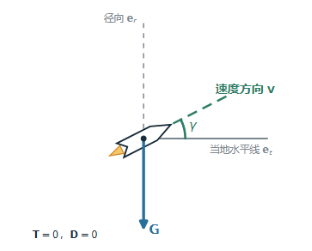
\includegraphics[width=\linewidth]{figure/1-3.png}
		\caption{无动力滑行阶段}
		\label{fig:1-3}
	\end{subfigure}
	\hfill
	\begin{subfigure}[b]{0.45\textwidth}
		\centering
		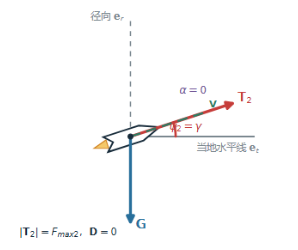
\includegraphics[width=\linewidth]{figure/1-4.png}
		\caption{二子级动力飞行阶段}
		\label{fig:1-4}
	\end{subfigure}
	\caption{各飞行阶段的受力、速度与推力方向关系}
	\label{fig:1}
\end{figure}
\subsubsection{DOP853数值求解}
对于运载火箭飞行过程中的各连续阶段，使用DOP853显式高阶Runge–Kutta方法。对常微分方程$\dot{\mathbf{x}} = \mathbf{f}(t,\mathbf{x})$，单步内部阶段量与更新式写为：
\begin{equation}
	\left\{
	\begin{aligned}
		\mathbf{k_i}
		&=
		\mathbf{f}(t_n+ c_ih_n,\mathbf{x_n}+h_n\sum\limits^{i-1}_{j=1}{a_{ij}}\mathbf{k}_j)\\
		\mathbf{x}_{n+1} 
		&= \mathbf{x}_n+h_n\sum\limits^s_{i=1}{b_i}\mathbf{k}_i
	\end{aligned}
	\right.
\end{equation}

由嵌入低阶公式估计局部误差en并自适应更新步长。相对误差容限取$10^{-9}$、绝对误差容限取$10^-12$，燃尽事件用质量零点定位，从而避免以固定步长近似燃尽时刻。
\begin{equation}
h_{n+1} = h_n clip \left[f_{min}, f_{max} , f_s(\frac{tol}{e_n})^{1/p+1}\right]
\end{equation}
其中clip()为阶段操作，将结果限定在$f_min$与$f_max$阈值之间。

则算法的整体流程为：积分一子级直到事件$g_1(\mathbf{x})=0$，执行质量跃变；以分离后状态积分60s滑行阶段；再以二子级全推力积分到$g_2(\mathbf{x})=0$。各段末状态作为下一段初状态，使位置、速度和时间轴连续衔接。
\subsubsection{问题一结果}
通过上述数值仿真，基准策略关键时刻与状态如\ref{tab:key_states}所示：
\begin{table}[htbp]
	\centering
	\caption{基准策略关键时刻与状态}
	\small
	\label{tab:key_states}
	\begin{tabular*}{\textwidth}{
			@{\extracolsep{\fill}}
			l
			S[table-format=3.2]
			S[table-format=3.2]
			S[table-format=-4.2]
			S[table-format=4.2]
			S[table-format=-2.2]
			S[table-format=3.2]
			@{}
		}
		\toprule
		时刻阶段
		& \multicolumn{1}{c}{$t$}
		& \multicolumn{1}{c}{$h$}
		& \multicolumn{1}{c}{$v_r$}
		& \multicolumn{1}{c}{$v_t$}
		& \multicolumn{1}{c}{$\gamma$}
		& \multicolumn{1}{c}{$m$} \\
		& \multicolumn{1}{c}{(\si{\second})}
		& \multicolumn{1}{c}{(\si{\kilo\metre})}
		& \multicolumn{1}{c}{(\si{\metre\per\second})}
		& \multicolumn{1}{c}{(\si{\metre\per\second})}
		& \multicolumn{1}{c}{(\si{\degree})}
		& \multicolumn{1}{c}{(\si{\tonne})} \\
		\midrule
		一子级燃尽 & 149.06 & 109.26 & 1944.27  & 2616.99 & 36.61 & 120.00 \\
		分离后     & 149.06 & 109.26 & 1944.27  & 2616.99 & 36.61 &  80.00 \\
		滑行结束   & 209.06 & 210.90 & 1445.86  & 2576.58 & 29.30 &  80.00 \\
		二子级燃尽 & 634.67 & 433.53 & -702.02  & 8520.57 & -0.69 &  18.00 \\
		\bottomrule
\end{tabular*}
\end{table}

由\ref{fig:2-1}可知，二子级燃料燃尽时高度已超过400km，且火箭切向速度8520.57 m/s高于该高度附近的圆轨道速度。基准策略只能给出完整轨迹，不能使有效载荷准确进入题定圆轨道。
\begin{figure}[htbp]
	\centering
	\begin{subfigure}[b]{0.45\textwidth}
		\centering
		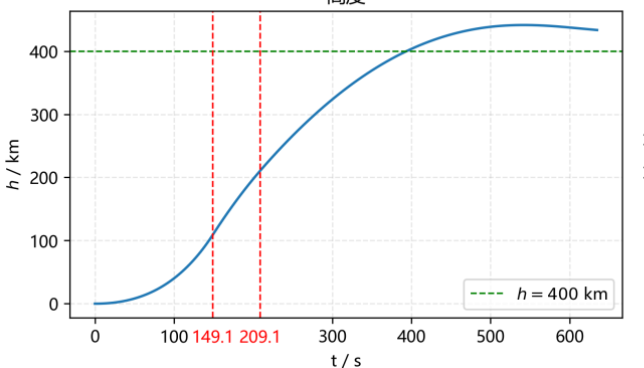
\includegraphics[width=\linewidth]{figure/2-1.png}
		\caption{高度}
		\label{fig:2-1}
	\end{subfigure}
	\hfill
	\begin{subfigure}[b]{0.45\textwidth}
		\centering
		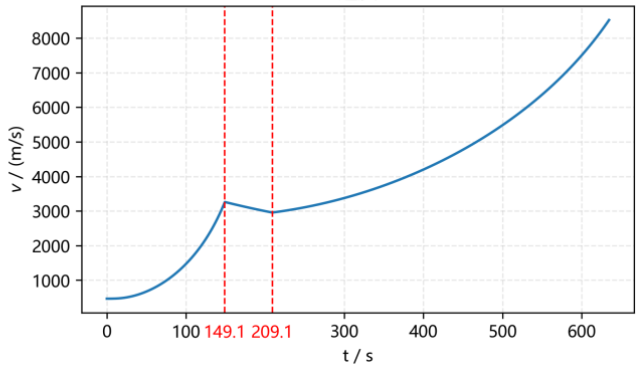
\includegraphics[width=\linewidth]{figure/2-2.png}
		\caption{速度}
		\label{fig:2-2}
	\end{subfigure}
	\begin{subfigure}[b]{0.45\textwidth}
		\centering
		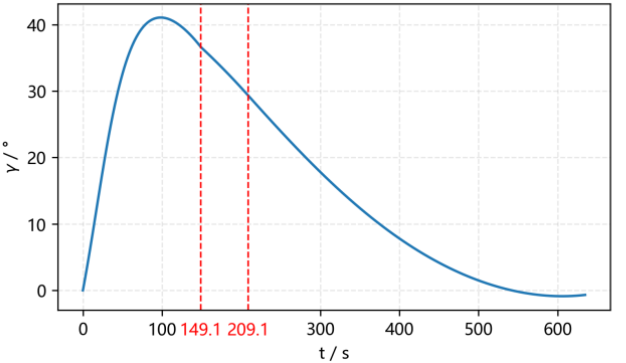
\includegraphics[width=\linewidth]{figure/2-3.png}
		\caption{飞机路径角}
		\label{fig:2-3}
	\end{subfigure}
	\hfill
	\begin{subfigure}[b]{0.45\textwidth}
		\centering
		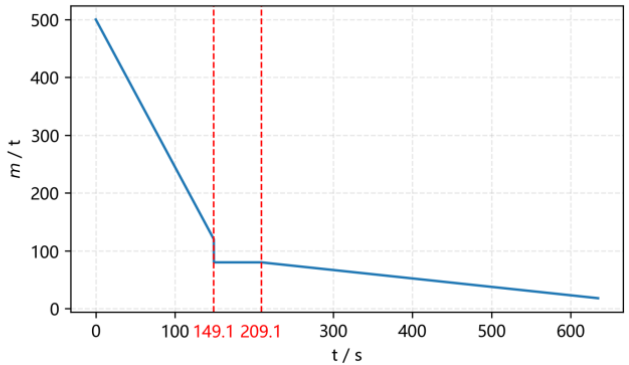
\includegraphics[width=\linewidth]{figure/2-4.png}
		\caption{总质量}
		\label{fig:2-4}
	\end{subfigure}
	\caption{基准控制策略下全过程状态曲线}
	\label{fig:2}
\end{figure}
\subsection{问题二模型建立及求解}
\label{sec:5.2}
\subsubsection{三参数打靶模型}
设一子级分离后的滑行时间为 $\tau$，二子级点火时刻的速度方向为
$\gamma_{\mathrm{ign}}$。二子级推力俯仰角以恒定速率 $k_2$ 变化，二子级工作时间为 $t_{c2}$，因此
\begin{equation}
	\psi_2(s)
	=
	\gamma_{\mathrm{ign}}+k_2s,
	\qquad
	0\leq s\leq t_{c2}.
	\label{eq:second_stage_pitch}
\end{equation}

目标圆轨道半径及其对应的圆轨道速度分别为
\begin{equation}
	\begin{aligned}
		r_{\mathrm{tar}}
		& =
		R_E+H, \\
		v_c
		&= 
		\sqrt{\frac{\mu}{r_{\mathrm{tar}}}}
	\end{aligned}
	\label{eq:target_orbit}
\end{equation}
从而定义待定参数向量与相应的三维打靶残差向量分别为
\begin{equation}
	\begin{aligned}
	\mathbf{p}
	& =
	\left[ \tau, k_2 , t_{c2} \right]^{\mathrm{T}},\\
	\mathbf{F}(\mathbf{p})
	&=
	\left[ 
	r_f-r_{\mathrm{tar}}, v_{r f} ,	v_{t f}-v_c  \right]^T
	\label{eq:parameter_vector}
\end{aligned}
\end{equation}

记滑行动力学的流映射为 $\Phi_c$，二子级动力学的流映射为
$\Phi_2$，则从一子级分离状态$\mathbf{x}_{\mathrm{sep}}$到终端状态 $\mathbf{x}_f$的参数映射可表示为
\begin{equation}
	\begin{aligned}
		\mathbf{x}_{\mathrm{ign}}
		&=
		\Phi_c
		\left(\tau;\mathbf{x}_{\mathrm{sep}}\right), \\
		\mathbf{x}_f
		&=
		\Phi_2
		\left(
		t_{c2};
		\mathbf{x}_{\mathrm{ign}},k_2
		\right).
	\end{aligned}
	\label{eq:state_flow_mapping}
\end{equation}

由于高度残差与速度残差的数量级不同，直接求根可能导致高度残差项在
数值计算中占主导。因此，对残差向量进行尺度缩放：
\begin{equation}
	\widetilde{\mathbf{F}}(\mathbf{p})
	=
	\left[
	\dfrac{r_f-r_{\mathrm{tar}}}{1000},
	\dfrac{v_{r,f}}{10},
	\dfrac{v_{t,f}-v_c}{10}
	\right]^T
	\label{eq:scaled_shooting_residual}
\end{equation}

\subsubsection{fsolve求解方法}
每给定一组$\mathbf{p}$，均按“滑行—二子级有动力飞行”顺序调用DOP853，得到终端残差。fsolve采用Powell混合算法，在Newton步与信赖域梯度步之间调整。其局部线性模型可写为
\begin{equation}
	\begin{aligned}
		\mathbf{d}_q
		&=
		\underset{
			\left\lVert\mathbf{D}\mathbf{d}\right\rVert
			\leq\Delta_q
		}{
			\operatorname{arg\,min}
		}
		\left\lVert
		\mathbf{F}(\mathbf{p}_q)
		+
		\mathbf{J}_{F}(\mathbf{p}_q)\mathbf{d}
		\right\rVert, \\
		\mathbf{p}_{q+1}
		&=
		\mathbf{p}_q+\mathbf{d}_q,
	\end{aligned}
	\label{eq:powell_hybrid}
\end{equation}
其中，$\mathbf{D}$ 为变量尺度矩阵，$\Delta_q$ 为第 $q$ 次迭代的信赖域半径，
$\mathbf{J}_{F}$ 为残差函数 $\mathbf{F}$ 关于参数向量 $\mathbf{p}$ 的 Jacobian
矩阵。

当未显式提供解析Jacobian时，程序用差分近似各列敏感度
\begin{equation}
	\mathbf{J}_{F,j}(\mathbf{p}_q)
	\approx
	\frac{
		\mathbf{F}\left(
		\mathbf{p}_q+\delta_j\mathbf{e}_j
		\right)
		-
		\mathbf{F}(\mathbf{p}_q)
	}{
		\delta_j
	},
	\label{eq:finite_difference_jacobian}
\end{equation}
其中，$\delta_j$ 为第 $j$ 个参数的差分步长，$\mathbf{e}_j$ 为第 $j$ 个坐标方向
上的单位向量。该 Jacobian 同时反映了滑行时间、俯仰角变化率和二子级工作时间对三个终端状态残差的耦合影响。

候选根需满足$\tau \geqslant 0 $、$0  \ \leq t_{c 2} \leqslant m_{p 2}I_{sp 2}g_0/F_{max 2}$，并以高精度积分重新计算终端残差。
为降低非线性方程对初值的敏感性，对滑行时间、俯仰角变化率和工作时间分别取3档初值，形成27组组合；收敛解还需满足工作时间不超过二子级理论燃尽时间且终端残差通过高精度复算。
\subsubsection{问题二结果}
\begin{table}[htbp]
	\centering
	\caption{问题二最优打靶参数与终端状态}
	\label{tab:optimal_shooting_results}
	\renewcommand{\arraystretch}{1.15}
	\begin{tabular*}{\textwidth}{
			@{\extracolsep{\fill}}
			lclc
			@{}
		}
		\toprule
		\multicolumn{1}{c}{项目}
		& 数值
		& \multicolumn{1}{c}{项目}
		& 数值 \\
		\midrule
		滑行时间 $\tau$/\si{\second}
		& 103.631602
		& 二子级工作时间 $t_{c2}$/\si{\second}
		& 398.048975 \\
		
		俯仰角变化率 $k_2$/(\si{\degree\per\second})
		& $-0.047365$
		& 总关机时刻 $t_f$/\si{\second}
		& 650.741657 \\
		
		终端高度 $h_f$/\si{\kilo\metre}
		& 400.000
		& 终端径向速度 $v_{r,f}$/(\si{\metre\per\second})
		& $\approx 0$ \\
		
		终端切向速度 $v_{t,f}$/(\si{\metre\per\second})
		& 7672.599
		& 剩余推进剂质量 $m_{p,f}$/\si{\kilogram}
		& 4014.72 \\
		
		多初值收敛数
		& $15/27$
		& 去重后有效根数
		& 1 \\
		\bottomrule
	\end{tabular*}
\end{table}
\begin{figure}[htbp]
	\centering
	\begin{subfigure}[b]{0.45\textwidth}
		\centering
		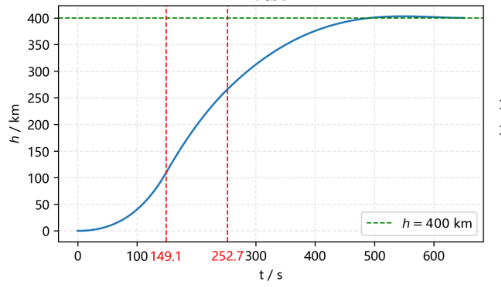
\includegraphics[width=\linewidth]{figure/3-1.png}
		\caption{高度}
		\label{fig:3-1}
	\end{subfigure}
	\hfill
	\begin{subfigure}[b]{0.45\textwidth}
		\centering
		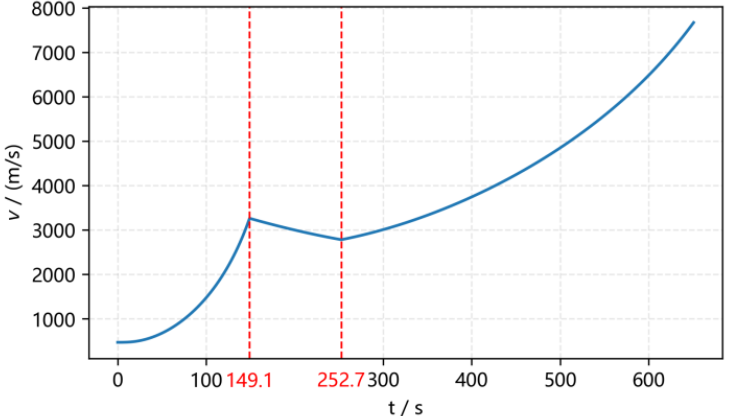
\includegraphics[width=\linewidth]{figure/3-2.png}
		\caption{速度}
		\label{fig:3-2}
	\end{subfigure}
	\begin{subfigure}[b]{0.45\textwidth}
		\centering
		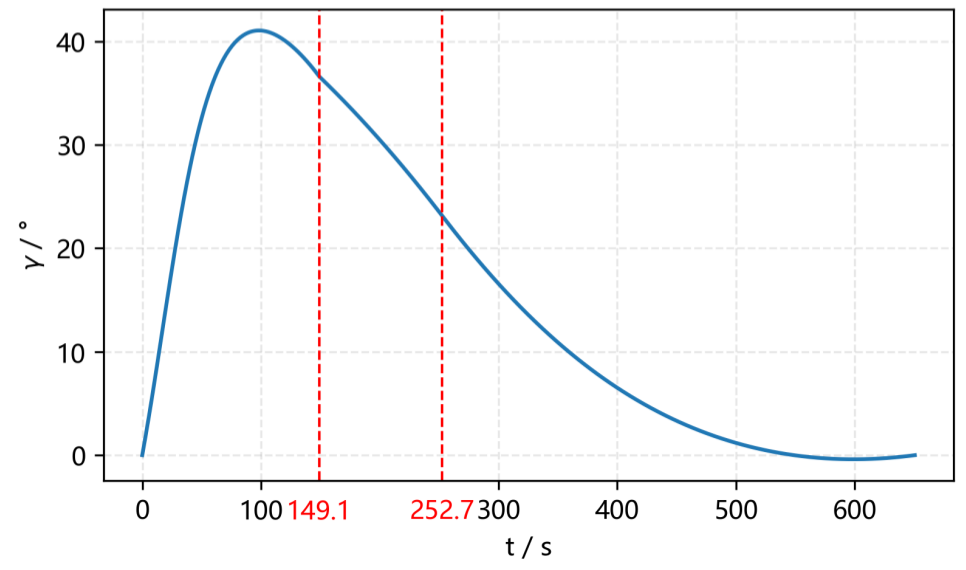
\includegraphics[width=\linewidth]{figure/3-3.png}
		\caption{飞机路径角}
		\label{fig:3-3}
	\end{subfigure}
	\hfill
	\begin{subfigure}[b]{0.45\textwidth}
		\centering
		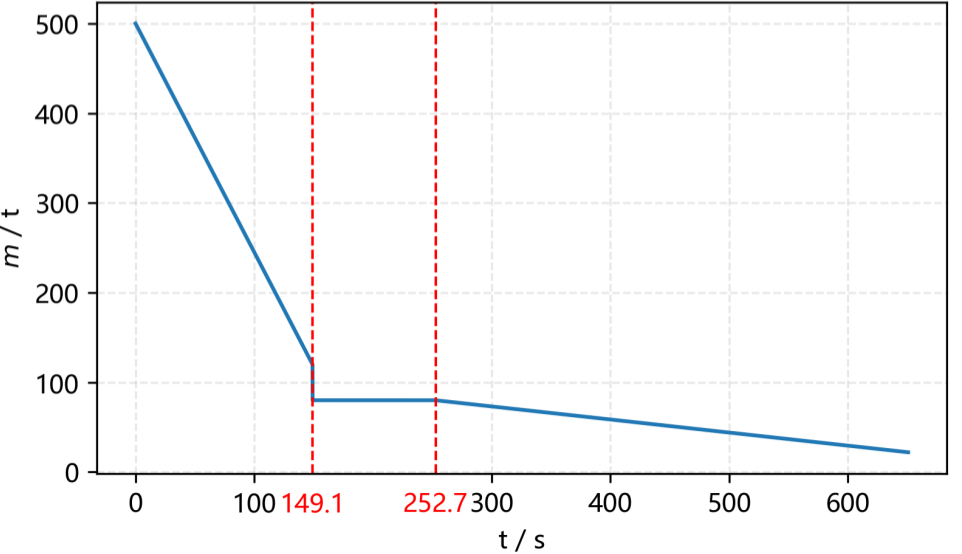
\includegraphics[width=\linewidth]{figure/3-4.png}
		\caption{总质量}
		\label{fig:3-4}
	\end{subfigure}
	\caption{基准控制策略下全过程状态曲线}
	\label{fig:3}
\end{figure}
终端高度、径向速度与切向速度同时满足400km圆轨道条件，且二子级尚余4014.72 kg推进剂。多初值结果去重后仅得到一个可接受根，说明该三参数控制形式下求解结果具有较好的初值稳定性。
\subsection{问题三模型建立及求解}
\label{sec:5.3}
\subsubsection{燃料最优控制模型}
二子级发动机保持额定推力 $F_{\max,2}$，且推进剂质量流率恒定，
因此推进剂消耗量与二子级工作时间成正比，即
\begin{equation}
	m_{\mathrm{fuel}}
	=
	\frac{F_{\max,2}}
	{I_{\mathrm{sp},2}g_0}
	t_{c2},
	\label{eq:fuel_consumption}
\end{equation}
其中，$I_{\mathrm{sp},2}$ 为二子级发动机比冲，$g_0$ 为标准重力加速度。

定义推力方向与速度方向之间的夹角为
\begin{equation}
	\alpha=\psi-\gamma,
	\label{eq:angle_of_attack}
\end{equation}
并对其施加如下约束：
\begin{equation}
	\lvert\alpha(t)\rvert
	\leq
	\alpha_{\max},
	\qquad
	\alpha_{\max}=15^\circ.
	\label{eq:angle_constraint}
\end{equation}
该约束与大气层外运载火箭轨迹优化相关文献采用的攻角上限处于相同数量级
~\cite{orgeira2022,civek2017}，本文仅将其作为附加的控制可实现性条件。

由此，轨迹优化问题可以表示为
\begin{equation}
	\begin{aligned}
		& \underset{\tau,\alpha(t),t_{c2}}{\min}
		\quad
		t_{c2} \\
		\text{s.t.}
		\quad
		& \mathbf{F}(\mathbf{p})=\mathbf{0}, \\
		& \lvert\alpha(t)\rvert
		\leq
		\alpha_{\max}.
	\end{aligned}
	\label{eq:trajectory_optimization}
\end{equation}

由于二子级额定推力和发动机比冲均为常数，推进剂消耗量是工作时间
$t_{c2}$ 的正比例函数。因此，最小化二子级工作时间与最小化推进剂消耗量
完全等价。

目标圆轨道由终端半径、径向速度和切向速度三个条件共同确定：
\begin{equation}
	\begin{cases}
		r(t_f)=R_E+H, \\[3pt]
		v_r(t_f)=0, \\[3pt]
		v_t(t_f)=
		\displaystyle
		\sqrt{\frac{\mu}{R_E+H}}.
	\end{cases}
	\label{eq:terminal_orbit_constraints}
\end{equation}

\subsubsection{控制参数化直接打靶}

在二子级局部时间区间$(0,t_{c 2})$上设置$K$个等距节点。节点间采用线性插值
在相邻控制节点 $t_j$ 和 $t_{j+1}$ 之间，采用线性插值确定推力与速度之间的夹角：
\begin{equation}
	\alpha(t)
	=
	\frac{t_{j+1}-t}{t_{j+1}-t_j}\alpha_j
	+
	\frac{t-t_j}{t_{j+1}-t_j}\alpha_{j+1},
	\qquad
	t_j\leq t\leq t_{j+1}.
	\label{eq:control_interpolation}
\end{equation}

对于包含 $K$ 个控制节点的离散模型，定义决策向量为
\begin{equation}
	\mathbf{z}_K
	=
	\begin{bmatrix}
		\tau &
		\alpha_0 &
		\cdots &
		\alpha_{K-1} &
		t_{c2}
	\end{bmatrix}^{\mathrm{T}}.
	\label{eq:decision_vector}
\end{equation}
对于每一组给定的决策向量 $\mathbf{z}_K$，从一子级分离状态开始，
依次对滑行段和二子级有动力飞行段的动力学方程进行正向积分，并将计算得到的
终端残差返回给优化器。该方法仅对控制量进行离散，而状态量仍通过微分方程
连续传播，因此称为控制参数化直接打靶法。

由于式~\eqref{eq:control_interpolation}中的线性插值系数均位于区间 $[0,1]$，
因此只要各控制节点满足
\begin{equation}
	-\alpha_{\max}
	\leq
	\alpha_j
	\leq
	\alpha_{\max},
	\qquad
	j=0,1,\ldots,K-1,
	\label{eq:node_angle_constraints}
\end{equation}
则整个时间区间内的夹角约束均能自动成立。

离散后的有限维非线性规划问题可以表示为
\begin{equation}
	\begin{aligned}
		& \underset{\mathbf{z}_K}{\min}
		\quad
		 J(\mathbf{z}_K)=t_{c2} \\
		\text{s.t.}
		\quad
		& \mathbf{F}(\mathbf{z}_K)=\mathbf{0}, \\
		& \mathbf{l}\leq\mathbf{z}_K\leq\mathbf{u},
	\end{aligned}
	\label{eq:discretized_nlp}
\end{equation}
其中，$\mathbf{l}$ 和 $\mathbf{u}$ 分别为决策变量的下界向量和上界向量。

\subsubsection{SLSQP求解与网格加密}
\label{sec:slsqp_mesh_refinement}

在第 $q$ 次迭代中，序列最小二乘二次规划（SLSQP）方法通过局部线性化约束，
构造如下二次规划子问题：
\begin{equation}
	\begin{aligned}
		\underset{\mathbf{d}}{\min}
		\quad
		&
		\nabla J\left(\mathbf{z}^{(q)}\right)^{\mathrm{T}}\mathbf{d}
		+
		\frac{1}{2}
		\mathbf{d}^{\mathrm{T}}
		\mathbf{B}^{(q)}
		\mathbf{d} \\
		\text{s.t.}
		\quad
		&
		\mathbf{F}\left(\mathbf{z}^{(q)}\right)
		+
		\mathbf{J}_F\left(\mathbf{z}^{(q)}\right)\mathbf{d}
		=
		\mathbf{0},
	\end{aligned}
	\label{eq:slsqp_subproblem}
\end{equation}
其中，$\mathbf{B}^{(q)}$ 为第 $q$ 次迭代中拉格朗日函数 Hessian 矩阵的
拟牛顿近似，$\mathbf{J}_F$ 为终端约束关于决策变量的 Jacobian 矩阵。

每次迭代首先通过有限差分计算目标函数和约束函数对决策变量的敏感度，
随后求解二次规划子问题，并通过线搜索确定更新步长。重复上述过程，
直至目标函数变化量、迭代步长和约束可行性误差同时达到给定的收敛阈值。

计算初始阶段采用 $K=9$ 个控制节点，并分别选取
\SI{0}{\second} 和 \SI{90}{\second} 作为滑行时间初值。随后将控制网格依次
加密至 $K=17$、$K=33$ 和 $K=65$ 个节点，并将上一层网格得到的最优控制
插值到新网格上，作为下一层优化的热启动初值。优化阶段的最大积分步长设置为
\SI{5}{\second}，最终采用 \SI{0.5}{\second} 的积分步长重新积分，以验证
优化结果。

具体求解流程如下：首先固定控制节点数，并给定滑行时间、夹角节点和二子级
工作时间的初始值；随后对每一组候选决策向量依次完成滑行段和有动力飞行段
积分，并计算目标函数以及三个缩放后的终端残差；SLSQP 更新决策向量后，
重新进行正向积分。算法收敛后，进一步执行边界检查、推进剂余量检查和
高精度积分复算。
\subsubsection{优化结果}
\begin{table}[htbp]
	\centering
	\caption{问题三网格加密结果与问题二结果对比}
	\label{tab:mesh_refinement_comparison}
	\small
	\renewcommand{\arraystretch}{1.15}
	\begin{tabular*}{\textwidth}{
			@{\extracolsep{\fill}}
			l
			S[table-format=2.0]
			S[table-format=3.6]
			S[table-format=3.6]
			S[table-format=4.3]
			S[table-format=1.2e-2]
			@{}
		}
		\toprule
		\multicolumn{1}{c}{方案}
		& \multicolumn{1}{c}{$K$}
		& \multicolumn{1}{c}{滑行时间/\si{\second}}
		& \multicolumn{1}{c}{工作时间/\si{\second}}
		& \multicolumn{1}{c}{剩余推进剂/\si{\kilogram}}
		& \multicolumn{1}{c}{缩放残差范数} \\
		\midrule
		问题二线性俯仰角程序
		& \multicolumn{1}{c}{--}
		& 103.631602
		& 398.048975
		& 4014.720
		& \multicolumn{1}{c}{--} \\
		
		直接打靶
		& 9
		& 27.066028
		& 394.649851
		& 4509.878
		& 3.76e-10 \\
		
		直接打靶
		& 17
		& 27.231056
		& 394.649593
		& 4509.916
		& 4.19e-10 \\
		
		直接打靶
		& 33
		& 27.383548
		& 394.649472
		& 4509.934
		& 6.47e-10 \\
		
		直接打靶
		& 65
		& 27.383720
		& 394.649418
		& 4509.941
		& 7.69e-11 \\
		\bottomrule
	\end{tabular*}
\end{table}
\begin{figure}[htbp]
	\centering
	\begin{subfigure}[b]{0.45\textwidth}
		\centering
		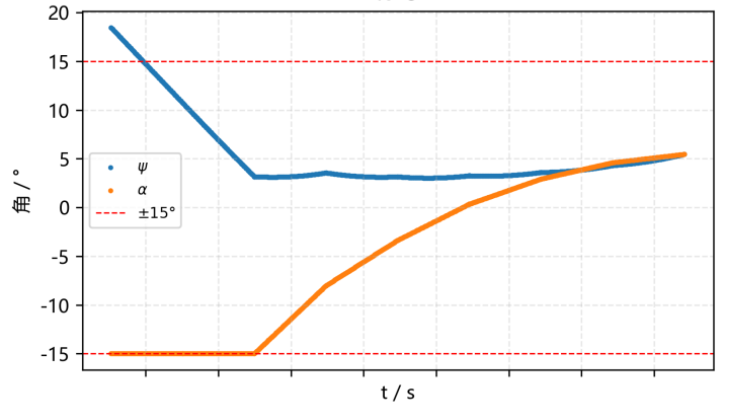
\includegraphics[width=\linewidth]{figure/4-1.png}
		\caption{K=9}
		\label{fig:4-1}
	\end{subfigure}
	\hfill
	\begin{subfigure}[b]{0.45\textwidth}
		\centering
		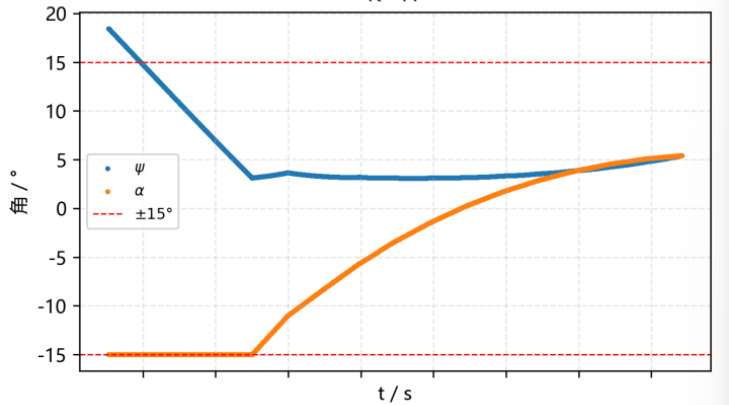
\includegraphics[width=\linewidth]{figure/4-2.png}
		\caption{K=17}
		\label{fig:4-2}
	\end{subfigure}
	\begin{subfigure}[b]{0.45\textwidth}
		\centering
		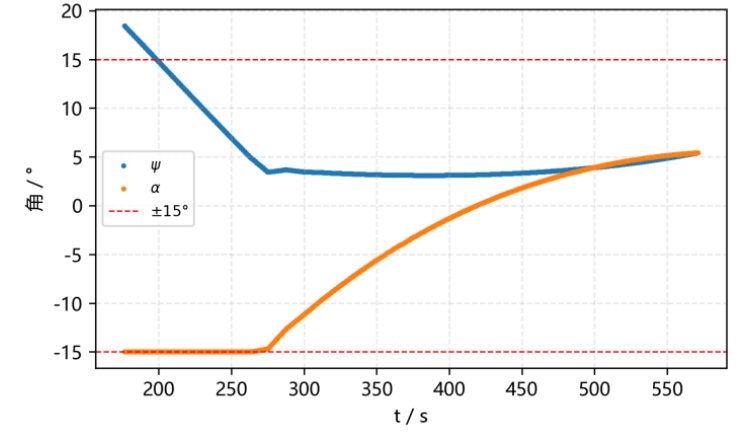
\includegraphics[width=\linewidth]{figure/4-3.png}
		\caption{K=33}
		\label{fig:4-3}
	\end{subfigure}
	\hfill
	\begin{subfigure}[b]{0.45\textwidth}
		\centering
		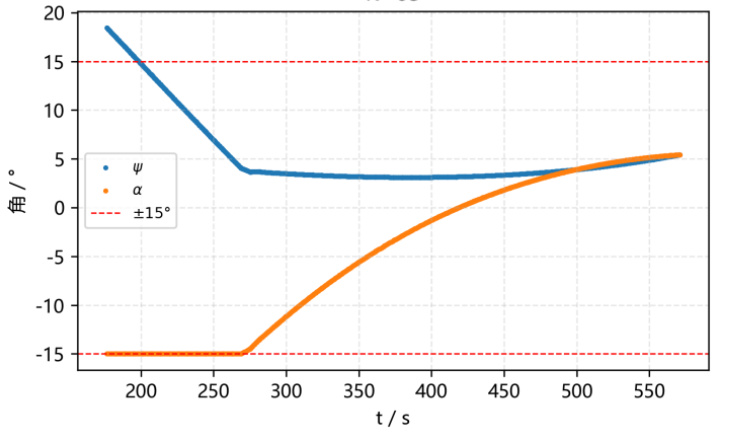
\includegraphics[width=\linewidth]{figure/4-4.png}
		\caption{K=65}
		\label{fig:4-4}
	\end{subfigure}
	\caption{基准控制策略下全过程状态曲线}
	\label{fig:4}
\end{figure}

控制节点加密后，工作时间与剩余推进剂逐步稳定。65节点结果较9节点仅多保留0.063 kg推进剂，表明控制离散误差已较小。最优夹角在二子级点火初期取−15°下界，随后逐渐进入约束内部，以较快降低径向速度并完成末段圆化。问题三较问题二多保留约495.22 kg推进剂。
\subsection{问题四模型建立及求解}
\label{sec:5.4}
\subsubsection{可节流动力学与燃料目标}
定义二子级节流比$u(t)=T(t)/F_{max 2}\in (0.6, 1)$。二子级状态方程中推力项统一替换为$uF_{max 2}$，则状态方程可以表示为
\begin{equation}
	\begin{cases}
		\dot{r}
		=
		v_r, \\[4pt]
		
		\dot{\theta}
		=
		\displaystyle\frac{v_t}{r}, \\[8pt]
		
		\dot{v}_r
		=
		\displaystyle
		\frac{v_t^2}{r}
		-
		\frac{\mu}{r^2}
		+
		\frac{
			u(t)F_{\max,2}\sin(\gamma+\alpha)
		}{m}, \\[10pt]
		
		\dot{v}_t
		=
		\displaystyle
		-\frac{v_rv_t}{r}
		+
		\frac{
			u(t)F_{\max,2}\cos(\gamma+\alpha)
		}{m}, \\[10pt]
		
		\dot{m}
		=
		\displaystyle
		-\frac{
			u(t)F_{\max,2}
		}{
			I_{\mathrm{sp},2}g_0
		}.
	\end{cases}
	\label{eq:throttled_second_stage_dynamics}
\end{equation}

令二子级实际工作时间为b，则推进剂消耗量由节流积分决定。定义等效满推力时间
\begin{equation}
	q
	=
	\int_0^b u(s)\,\mathrm{d}s,
	\label{eq:equivalent_full_thrust_time}
\end{equation}
相应的推进剂消耗量为
\begin{equation}
	m_{\mathrm{fuel}}
	=
	\frac{F_{\max,2}}
	{I_{\mathrm{sp},2}g_0}
	q.
	\label{eq:throttled_fuel_consumption}
\end{equation}
\begin{figure}[htbp]
	\centering
	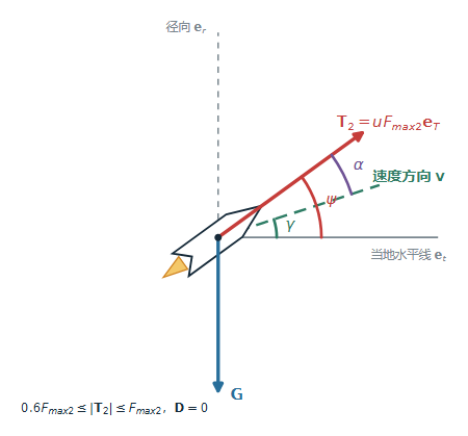
\includegraphics[width=0.8\textwidth]{figure/5.png}
	\caption{问题四二子级可节流飞行的受力与控制关系}
	\label{fig:5}
\end{figure}
\subsubsection{双控制参数化模型}
\label{sec:dual_control_parameterization}

在相同的 $K$ 个等距控制节点上分别设置推力与速度夹角 $\alpha_j$ 和节流比
$u_j$，并在相邻节点之间进行分段线性插值。由于节流比采用分段线性插值，
在均匀节点条件下，其平均值可以由梯形公式精确计算：
\begin{equation}
	\overline{u}
	=
	\frac{
		\displaystyle
		\frac{1}{2}u_0
		+
		\sum_{j=1}^{K-2}u_j
		+
		\frac{1}{2}u_{K-1}
	}{
		K-1
	},
	\qquad
	b=\frac{q}{\overline{u}},
	\label{eq:average_throttle}
\end{equation}
其中，$\overline{u}$ 为平均节流比，$q$ 为等效满推力时间，$b$ 为二子级
发动机的实际工作时间。

为改善不同决策变量之间的尺度差异，定义缩放后的决策向量为
\begin{equation}
	\mathbf{z}
	=
	\begin{bmatrix}
		\dfrac{\tau}{100} &
		\alpha_0 &
		\cdots &
		\alpha_{K-1} &
		u_0 &
		\cdots &
		u_{K-1} &
		\dfrac{q}{400}
	\end{bmatrix}^{\mathrm{T}}.
	\label{eq:scaled_dual_control_vector}
\end{equation}

实际工作时间由 $b=q/\overline{u}$ 反算得到，因此任意候选决策向量对应的
推进剂消耗量均与其节流积分保持一致。问题四的有限维优化模型可以表示为
\begin{equation}
	\begin{aligned}
		& \underset{\mathbf{z}}{\min}
		\quad
		 J(\mathbf{z})=q \\
		\text{s.t.}
		\quad
		& \mathbf{F}(\mathbf{z})=\mathbf{0}, \\
		& \lvert\alpha_j\rvert\leq 15^\circ,
		\qquad j=0,1,\ldots,K-1, \\
		& 0.6\leq u_j\leq 1,
		\qquad j=0,1,\ldots,K-1, \\
		& 0\leq\tau\leq\tau_{\max}, \\
		& 0<q\leq
		\frac{
			m_{p2}I_{\mathrm{sp},2}g_0
		}{
			F_{\max,2}
		}.
	\end{aligned}
	\label{eq:dual_control_optimization}
\end{equation}

其中，三项等式约束分别对应高度为 \SI{400}{\kilo\metre} 的目标圆轨道半径、
零径向速度和目标切向速度。SLSQP 的求解结构与问题三相同，但决策变量的维数
增加至
\begin{equation}
	\dim(\mathbf{z})=2K+2.
\end{equation}

对于缩放后的决策变量，目标函数关于最后一个分量的梯度为 $400$，关于其余
分量的梯度均为 $0$；终端约束的 Jacobian 矩阵采用有限差分方法计算。
在 $K=9$ 个控制节点时，分别采用全推力、$80\%$ 推力和 $60\%$ 推力作为
节流比初值。随后将控制网格依次加密至 $K=17$ 和 $K=33$ 个节点，并使用
上一层网格的优化结果进行插值，以构造下一层优化的热启动初值。

对于每个收敛的候选解，均重新计算节流积分、剩余推进剂质量和终端状态，
并在相同节点数下与问题三的计算结果进行比较。

\subsubsection{求解结果与节流判定}
不同控制节点数下的网格加密结果如\ref{tab:problem4_mesh_results}所示。

\begin{table}[htbp]
	\centering
	\caption{问题四网格加密结果}
	\label{tab:problem4_mesh_results}
	\small
	\renewcommand{\arraystretch}{1.15}
	\begin{tabular*}{\textwidth}{
			@{\extracolsep{\fill}}
			c
			S[table-format=2.0]
			S[table-format=3.6]
			S[table-format=3.6]
			c
			S[table-format=4.3]
			S[table-format=1.2e-2]
			@{}
		}
		\toprule
		{$K$}
		& {\makecell{滑行时间\\(\si{\second})}}
		& {\makecell{工作时间\\(\si{\second})}}
		& {\makecell{等效满推力时间\\(\si{\second})}}
		& {节流范围}
		& {\makecell{剩余推进剂\\(\si{\kilogram})}}
		& {缩放残差范数} \\
		\midrule
		9
		& 27.0660
		& 394.650
		& 394.450
		& $1.000\sim1.000$
		& 4509.878
		& 2.17e-10 \\
		
		17
		& 27.227
		& 394.650
		& 394.650
		& $1.000\sim1.000$
		& 4509.916
		& 9.48e-10 \\
		
		33
		& 27.385
		& 394.649
		& 394.649
		& $1.000\sim1.000$
		& 4509.933
		& 1.90e-10 \\
		\bottomrule
	\end{tabular*}
\end{table}
三组9节点初值均收敛到同一全程满推力结构，17和33节点加密后节流比仍为1。由于此时q=b，问题四在相同网格上的目标值与问题三一致。该结果表明，在当前动力学、圆轨道终端条件和夹角约束下，降低推力延长飞行时间带来的重力损失超过其可能产生的控制收益，因此允许节流并未进一步减少推进剂消耗。该结论是多初值和网格加密支持的最优候选，不等同于严格的全局最优性证明。
\begin{figure}[htbp]
	\centering
	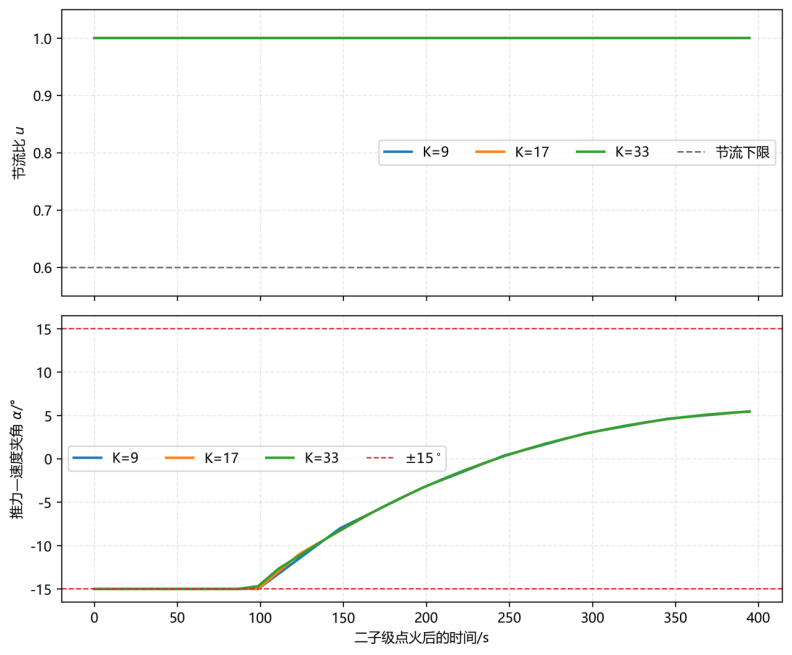
\includegraphics[width=0.8\textwidth]{figure/6.png}
	\caption{问题四二子级可节流飞行的受力与控制关系}
	\label{fig:6}
\end{figure}
\begin{figure}[htbp]
	\centering
	\begin{subfigure}[b]{0.45\textwidth}
		\centering
		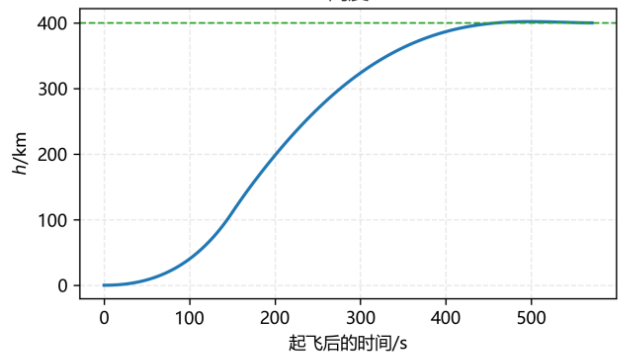
\includegraphics[width=\linewidth]{figure/7-1.png}
		\caption{高度}
		\label{fig:7-1}
	\end{subfigure}
	\hfill
	\begin{subfigure}[b]{0.45\textwidth}
		\centering
		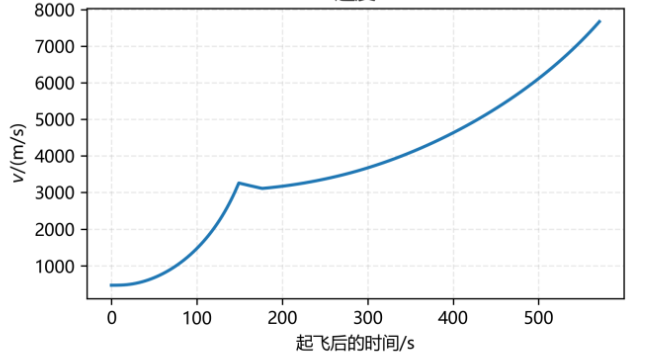
\includegraphics[width=\linewidth]{figure/7-2.png}
		\caption{速度}
		\label{fig:7-2}
	\end{subfigure}
	\begin{subfigure}[b]{0.45\textwidth}
		\centering
		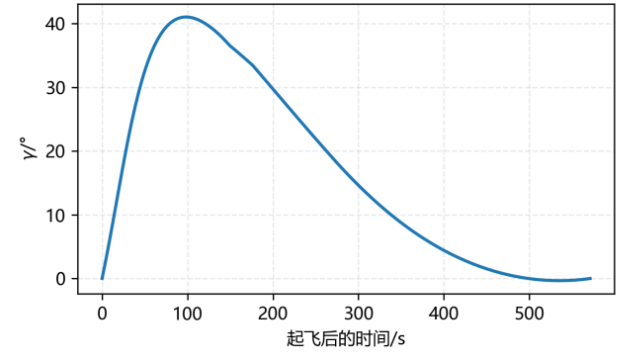
\includegraphics[width=\linewidth]{figure/7-3.png}
		\caption{飞机路径角}
		\label{fig:7-3}
	\end{subfigure}
	\hfill
	\begin{subfigure}[b]{0.45\textwidth}
		\centering
		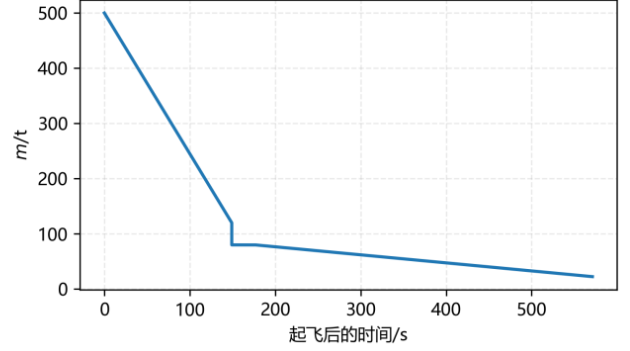
\includegraphics[width=\linewidth]{figure/7-4.png}
		\caption{总质量}
		\label{fig:7-4}
	\end{subfigure}
	\caption{基准控制策略下全过程状态曲线}
	\label{fig:7}
\end{figure}
\subsubsection{数值敏感性检验}
由\ref{tab:step_size_sensitivity}可知，在六种积分最大步长下，剩余推进剂
质量均保持为 \SI{4509.9335}{\kilogram}。终端高度的绝对误差均小于
\SI{2e-7}{\metre}，缩放残差范数均保持在 $10^{-10}$ 数量级。
因此，计算结果对积分最大步长的变化不敏感，说明所得结论不依赖于某一特定的
最大步长设置。
\begin{table}[htbp]
	\centering
	\caption{问题四中33节点解对积分最大步长的敏感性}
	\label{tab:step_size_sensitivity}
	\footnotesize
	\renewcommand{\arraystretch}{1.15}
	\begin{tabular*}{\textwidth}{
			@{\extracolsep{\fill}}
			S[table-format=1.2]
			S[table-format=4.4]
			S[table-format=-1.2e-1]
			S[table-format=-1.2e-2]
			S[table-format=-1.2e-2]
			S[table-format=1.2e-2]
			@{}
		}
		\toprule
		\multicolumn{1}{c}{\makecell{最大步长\\(\si{\second})}}
		& \multicolumn{1}{c}{\makecell{剩余推进剂\\(\si{\kilogram})}}
		& \multicolumn{1}{c}{\makecell{高度误差\\(\si{\metre})}}
		& \multicolumn{1}{c}{\makecell{径向速度误差\\(\si{\metre\per\second})}}
		& \multicolumn{1}{c}{\makecell{切向速度误差\\(\si{\metre\per\second})}}
		& \multicolumn{1}{c}{\makecell{缩放残差\\范数}} \\
		\midrule
		0.10 & 4509.934 & -1.62e-7 & -3.23e-10 & -9.48e-10 & 1.90e-10 \\
		0.25 & 4509.934 & -1.19e-7 &  1.44e-11 &  1.73e-11 & 1.19e-10 \\
		0.50 & 4509.934 & -1.23e-7 & -3.50e-11 & -5.28e-11 & 1.23e-10 \\
		1.00 & 4509.934 & -1.19e-7 & -6.47e-12 & -2.36e-11 & 1.19e-10 \\
		2.00 & 4509.934 & -1.30e-7 & -2.47e-11 & -3.18e-11 & 1.30e-10 \\
		5.00 & 4509.934 & -1.29e-7 & -2.09e-11 & -2.27e-11 & 1.29e-10 \\
		\bottomrule
	\end{tabular*}
\end{table}
\section{模型评价与推广}
\subsection{模型优点}
模型在统一的惯性极坐标框架内处理中心引力、地球自转初速度、旋转大气阻力、变质量和级间质量跃变，避免了不同问题采用不一致状态定义。问题二采用多初值非线性打靶，问题三、四采用控制参数化、网格加密和独立高精度复算，数值结果能够相互衔接。问题四重新定义燃料目标，避免将可节流条件下的工作时间误当作耗油量。
\subsubsection{模型不足}
本文采用二维质点模型和指数大气，未描述姿态角速度、发动机摆角速率、节流速率、结构载荷、动压与热流等路径约束；15°夹角上限为文献支持的附加建模条件，并非本题火箭的已知硬件极限。SLSQP属于局部优化方法，多初值与网格加密只能增强候选解可信度，不能给出全局最优性证明。补充的庞特里亚金极小值原理单点打靶在现行径向—切向模型下未达到残差验收标准，因此未将其旧结果用于本文结论。进一步研究可采用多重打靶或伪谱法，并加入三维地球模型和工程路径约束。
\subsection{模型推广}
本文的分阶段动力学与控制参数化框架不依赖某一组固定火箭参数。替换各级质量、推力、比冲和气动参数后，可用于其他多级运载器的基准轨迹计算与入轨控制设计；增加目标轨道倾角、分离方位角及三维速度分量后，可推广至非赤道发射和三维轨迹优化。燃料目标还可与动压、过载和热流峰值组成多目标函数，为工程设计提供效率与安全之间的权衡方案。
\section{AI工具使用说明}\label{sec:7}
研究过程中使用生成式人工智能工具辅助资料核对、文字表达和公式排版。动力学方程、约束条件、程序实现与数值结果均以题目资料和团队代码为依据重新计算，并由团队成员人工复核。AI工具信息与详细使用情况见\ref{tab:AI_usage}。
\begin{table}[htbp]
	\centering
	\caption{AI工具使用说明}\label{tab:AI_usage}
	\begin{tabularx}{\textwidth}{cX}
		\toprule
		项目 & 说明\\
		\midrule
		工具名称 & Kimi\\
		版本或型号 & Kimi K3 \\ 
		工具用途 & 资料核对、语言润色、公式及Word排版辅助\\
		结果核验 & 动力学方程、程序和数值结果均依据团队代码重新计算并人工复核\\
		\bottomrule
	\end{tabularx}
\end{table}
\clearpage
\begin{thebibliography}{99}
	\bibitem{hairer1993}
	Hairer E, N{\o}rsett S P, Wanner G.
	\newblock \textit{Solving Ordinary Differential Equations I: Nonstiff Problems}[M].
	\newblock 2nd ed. Berlin: Springer, 1993.
	
	\bibitem{more1980}
	Mor\'e J J, Garbow B S, Hillstrom K E.
	\newblock \textit{User Guide for MINPACK-1}[R].
	\newblock Argonne National Laboratory Report ANL-80-74, 1980.
	
	\bibitem{kraft1988}
	Kraft D.
	\newblock \textit{A Software Package for Sequential Quadratic Programming}[R].
	\newblock DFVLR-FB 88-28, 1988.
	
	\bibitem{orgeira2022}
	Orgeira-Crespo P, et al.
	\newblock Optimization of the Conceptual Design of a Multistage Rocket Launcher[J].
	\newblock \textit{Aerospace}, 2022, 9(6): 286.
	\newblock DOI: \url{https://doi.org/10.3390/aerospace9060286}.
	
	\bibitem{civek2017}
	Civek-Co\c{s}kun E, \"Ozg\"oren M K.
	\newblock Space Launch Vehicle Design with Simultaneous Optimization of
	Thrust Profile and Trajectory[C]//
	\newblock \textit{AIAA SPACE and Astronautics Forum and Exposition}.
	2017: AIAA 2017-5333.
	\newblock DOI: \url{https://doi.org/10.2514/6.2017-5333}.
	
	\bibitem{betts2010}
	Betts J T.
	\newblock \textit{Practical Methods for Optimal Control and Estimation
		Using Nonlinear Programming}[M].
	\newblock 2nd ed. Philadelphia: SIAM, 2010.
	
\end{thebibliography}

\begin{appendixx}
%\section{支撑材料}
%\begin{figure}[htbp]
%	\centering
%	\includegraphics[width=0.4\textwidth]{example-image.pdf}
%	\caption{支撑材料目录}
%	\label{fig:example}
%\end{figure}
\section{工具函数的Python脚本（核心部分）}
\begin{python}[
	frame=single,
	breaklines=true,
	breakatwhitespace=false,
	caption={utils.py},
	label={lst:constant}
	]
import time
import logging
from pathlib import Path
import numpy as np
from PIL import Image
logging.getLogger('tifffile').addFilter(lambda record: 'not a valid EXTRASAMPLE' not in record.getMessage())
SMIN, SMAX = 0.0, 255.0
IMG_DIR = Path('../参考文献及测试图片/standard_test_images')
def load_gray(path):
    try:
        return np.asarray(Image.open(path).convert('L'), float)
    except Exception:
        import tifffile
        a = tifffile.imread(path)
        if a.ndim == 3:
            a = a[..., 0]
        return a.astype(float)
#椒盐噪声生成，对称：p = q = r/2
def add_salt_pepper_noise(img, ratio, rng):
    y = img.astype(float).copy()
    r = rng.random(y.shape)
    y[r < ratio / 2] = SMIN
    y[r > 1 - ratio / 2] = SMAX
    return y
# 自适应中值滤波。返回 (输出图 out, 噪声候选掩码 omega)
def amf_detect(y, wmax=9):
    from scipy.ndimage import rank_filter
    y = y.astype(float)
    edges = list(range(3, wmax + 1, 2))            # 3,5,...,wmax
    zmed_layer = [rank_filter(y, size=w, rank=w * w // 2) for w in edges]
    zmin_layer = [rank_filter(y, size=w, rank=0) for w in edges]
    zmax_layer = [rank_filter(y, size=w, rank=w * w - 1) for w in edges]
    out = y.copy()
    done = np.zeros(y.shape, bool)
    for w, zmed, zmin, zmax in zip(edges, zmed_layer, zmin_layer, zmax_layer):
        not_extreme = (zmin < y) & (y < zmax)       # 干净像素
        replaceable = (~not_extreme) & (zmin < zmed) & (zmed < zmax)
        decide = ~done & (not_extreme | replaceable)
        out[replaceable] = zmed[replaceable]
        done |= decide
        if done.all():
            break
    todo = ~done
    if todo.any():
        out[todo] = zmed_layer[-1][todo]             # 最大窗口中值兜底
    omega = ((y == SMIN) | (y == SMAX)) & (out != y)
    return out, omega
# 势函数及导数
def make_potential(name, alpha):
    # sqrt(t^2 + alpha)
    if name == 'sqrt':
        return (lambda t: np.sqrt(t * t + alpha),
                lambda t: t / np.sqrt(t * t + alpha))
    # |t|^alpha, 1 < alpha <= 2
    if name == 'power':
        def dphi(t):
            return np.sign(t) * alpha * np.abs(t) ** (alpha - 1)
        return lambda t: np.abs(t) ** alpha, dphi
    # log(cosh(alpha t)) / alpha
    if name == 'logcosh':
        a = alpha
        def phi(t):
            at = a * np.abs(t)
            return (at + np.log1p(np.exp(-2 * at)) - np.log(2.0)) / a
        return phi, (lambda t: np.tanh(a * t))
    # |t|/alpha - log(1 + |t|/alpha)
    if name == 'log':
        def phi(t):
            at = np.abs(t) / alpha
            return at - np.log1p(at)
        def dphi(t):
            at = np.abs(t)
            return np.sign(t) * at / (alpha * (alpha + at))
        return phi, dphi
    # Huber
    if name == 'huber':
        def phi(t):
            at = np.abs(t)
            return np.where(at <= alpha, t * t / (2 * alpha), at - alpha / 2)
        return phi, (lambda t: np.clip(t / alpha, -1.0, 1.0))
    return None
def smooth_abs(mu):
    return lambda t: np.sqrt(t * t + mu * mu), lambda t: t / np.sqrt(t * t + mu * mu)
# 四邻域无向边
def _edges(shape):
    m, n = shape
    return [
        ((slice(1, m), slice(0, n)), (slice(0, m - 1), slice(0, n))),   # 上邻 q=(i-1,j)
        ((slice(0, m - 1), slice(0, n)), (slice(1, m), slice(0, n))),   # 下邻 q=(i+1,j)
        ((slice(0, m), slice(1, n)), (slice(0, m), slice(0, n - 1))),   # 左邻 q=(i,j-1)
        ((slice(0, m), slice(0, n - 1)), (slice(0, m), slice(1, n))),   # 右邻 q=(i,j+1)
    ]
# 构造简化泛函 G 的光滑化版本
def make_problem(y, omega, beta, phi, dphi, mu):
    psi, dpsi = smooth_abs(mu)
    edges = [(p, q, np.where(omega[q], 1.0, 2.0)) for p, q in _edges(y.shape)]
    def v_image(u):
        v = u.copy()
        v[~omega] = y[~omega]
        return v
    def objective(u):
        v = v_image(u)
        val = psi(u[omega] - y[omega]).sum()
        for (pr, pc), (qr, qc), w in edges:
            diff = u[pr, pc] - v[qr, qc]
            val += 0.5 * beta * (w * phi(diff) * omega[pr, pc]).sum()
        return val
    def gradient(u):
        v = v_image(u)
        g = np.zeros_like(u)
        g[omega] = dpsi(u[omega] - y[omega])
        for (pr, pc), (qr, qc), _ in edges:
            g[pr, pc] += beta * dphi(u[pr, pc] - v[qr, qc]) * omega[pr, pc]
        return g
    return objective, gradient
# 逐元素截断到 [SMIN, SMAX]
def project(u):
    return np.clip(u, SMIN, SMAX)
# BB 步长 + Armijo 线搜索的投影梯度
def projected_gradient(f, g, u0, maxit=80, tol=1e-4):
    u = project(u0)
    fu, gu = f(u), g(u)
    u_prev, g_prev = u.copy(), gu.copy()
    for k in range(1, maxit + 1):
        residual = np.max(np.abs(u - project(u - gu))) / max(1.0, np.max(np.abs(u)))
        if residual <= tol:
            return u, k - 1
        if k >= 2:
            s = u - u_prev
            z = gu - g_prev
            sz = (s * z).sum()
            eta = (s * s).sum() / sz if sz > 1e-30 else 1.0
        else:
            eta = 1.0
        step = float(np.clip(eta, 1e-10, 1e10))
        c1, decay = 1e-4, 0.5
        while step > 1e-20:
            un = project(u - step * gu)
            fn = f(un)
            if fn <= fu + c1 * (gu * (un - u)).sum():
                break
            step *= decay
        else:
            return u, k - 1
        gn = g(un)
        u_prev, g_prev, u, fu, gu = u, gu, un, fn, gn
    return u, k
# 光滑延拓mu_j = mu0 * rho^j，共 n_layers 层, 投影梯度恢复
def restore(y, omega, beta=20.0, pot='sqrt', alpha=1e-4, mu0=1.0, rho=0.1,
            n_layers=4, maxit=80, tol=1e-4):
    phi, dphi = make_potential(pot, alpha)
    u = y.copy()
    total = 0
    mu = mu0
    for _ in range(n_layers):
        f, g = make_problem(y, omega, beta, phi, dphi, mu=mu)
        u, k = projected_gradient(f, g, u, maxit=maxit, tol=tol)
        total += k
        mu *= rho
    return u, total
# 加载 → 加噪 → AMF 检测 → 恢复，带分段计时
def run_pipeline(img_name, ratio, seed=0, restore_kw=None, wmax=None):
    rng = np.random.default_rng(seed)
    x = load_gray(IMG_DIR / f'{img_name}.tif')
    y = add_salt_pepper_noise(x, ratio, rng)
    t0 = time.perf_counter()
    amf_out, omega = amf_detect(y, wmax=wmax or (9 if ratio >= 0.4 else 7))
    t1 = time.perf_counter()
    if restore_kw is None:
        restore_kw = {}
    u, iters = restore(y, omega, **restore_kw)
    t2 = time.perf_counter()
    return x, y, amf_out, omega, u, iters, (t1 - t0, t2 - t1)
def mse(xhat, x):
    return np.mean((xhat - x) ** 2)
def psnr(xhat, x):
    return 10 * np.log10(SMAX ** 2 / mse(xhat, x))
def snr(xhat, x):
    return 20 * np.log10(np.linalg.norm(x) / np.linalg.norm(xhat - x))
\end{python}
\section{问题一求解的Python脚本（核心部分）}
\begin{python}[
	frame=single,
	breaklines=true,
	breakatwhitespace=false,
	caption={prob1.py},
	label={lst:constant}
	]
import sys
from pathlib import Path
import numpy as np
from PIL import Image as PILImage
from utils import IMG_DIR, load_gray, psnr, run_pipeline, snr
POT, ALPHA = 'sqrt', 1e-4          # 问题一主模型势函数
BETA = 20.0                        # 正则化强度
def run(img_name, ratio, seed=0):
    x, y, amf_out, omega, u, iters, (t_det, t_opt) = run_pipeline(img_name, ratio, seed=seed,restore_kw=dict(beta=BETA, pot=POT, alpha=ALPHA, n_layers=5))
    rows = [
        ('noisy', y, psnr(y, x), snr(y, x), 0.0),
        ('amf', amf_out, psnr(amf_out, x), snr(amf_out, x), t_det),
        ('restored', u, psnr(u, x), snr(u, x), t_opt),
    ]
    return rows
if __name__ == '__main__':
    if len(sys.argv) > 1:
        names = sys.argv[1:]
    else:
        names = sorted(p.stem for p in IMG_DIR.glob('*.tif'))
    seed = 0
    summary = []
    saved_grids = set()
    for n in names:
        for r in (0.3, 0.5):
            rows = run(n, r, seed=seed)
            for name, _, p, _, elapsed in rows:
                summary.append((n, r, name, p, elapsed))
    print(f'summary')
\end{python}
\section{问题二求解的Python脚本（核心部分）}
\begin{python}[
	frame=single,
	breaklines=true,
	breakatwhitespace=false,
	caption={prob2.py},
	label={lst:constant}
	]
from pathlib import Path
from utils import psnr, run_pipeline, snr
import numpy as np
from utils import IMG_DIR, load_gray, make_potential
BETA_GRID = [5.0, 10.0, 20.0, 30.0, 50.0]
CALIB_KW = dict(n_layers=2, maxit=25, tol=1e-3)
NOISE_RATIOS = (0.3, 0.5)
SEED = 0
IMAGE_NAMES = sorted(p.stem for p in IMG_DIR.glob('*.tif'))
VAL_NAMES = IMAGE_NAMES[:3]
TEST_NAMES = IMAGE_NAMES[3:]
POTENTIALS = ['sqrt', 'power', 'logcosh', 'log', 'huber']
ALPHA_FIXED = {'sqrt': 1e-06, 'power': 1.1, 'logcosh': 2.5, 'log': 0.9, 'huber': 1.0}
T_FAR = 10
CANDIDATES = {
    'sqrt':    [1e-6, 1e-4, 1e-2, 1.0],
    'power':   [1.1,1.2, 1.3, 1.5, 1.8],
    'logcosh': [1.0, 1.5, 2.0, 2.5],
    'log':     [0.8,0.9, 1.0, 1.3],
    'huber':   [1.0, 1.3, 1.5, 2],
}
def edge_samples(img_name):
    x = load_gray(IMG_DIR / f'{img_name}.tif')
    d = np.concatenate([np.abs(np.diff(x, axis=0)).ravel(),np.abs(np.diff(x, axis=1)).ravel()])
    return d, d[d >= T_FAR]
def explore_alpha(img_name):
    d, t = edge_samples(img_name)
    for pot, cands in CANDIDATES.items():
        for a in cands:
            phi, dphi = make_potential(pot, a)
            rel = np.abs(phi(t) - t) / t
            ddev = np.abs(dphi(t) - 1.0)
            h = 1e-3 * np.maximum(t, 1.0)
            num = np.abs(dphi(t) - (phi(t + h) - phi(t - h)) / (2 * h))
        print()
def psnr_batch(pot, alpha, beta, names, ratio):
    psnrs = []
    for n in names:
        x, y, _, omega, u, _, _ = run_pipeline(
            n, ratio, seed=SEED,
            restore_kw=dict(beta=beta, pot=pot, alpha=alpha, **CALIB_KW))
        psnrs.append(psnr(np.where(omega, u, y), x))
    return float(np.mean(psnrs))
# 对单一 pot 在单噪声率上做beta搜索。
def find_best_beta(pot, ratio):
    best_v, best_b = -np.inf, BETA_GRID[0]
    for b in BETA_GRID:
        v = psnr_batch(pot, ALPHA_FIXED[pot], b, VAL_NAMES, ratio)
        if v > best_v:
            best_v, best_b = v, b
    return ALPHA_FIXED[pot], best_b, best_v
def run_one(img_name, ratio, pot, alpha, beta):
    x, y, _, omega, u, iters, (t_det, t_opt) = run_pipeline(
        img_name, ratio, seed=SEED,
        restore_kw=dict(beta=beta, pot=pot, alpha=alpha))
    xhat = np.where(omega, u, y)
    return dict(name=img_name, ratio=ratio, pot=pot, alpha=alpha,
                beta=beta, iters=iters, t_det=t_det, t_opt=t_opt,
                psnr=psnr(xhat, x), snr=snr(xhat, x))
def main():
    OUT_DIR.mkdir(exist_ok=True)
    # explore_alpha('lena_gray_512')
    calib = {}
    for pot in POTENTIALS:
        calib[pot] = {}
        for r in NOISE_RATIOS:
            a, b, v = find_best_beta(pot, r)
            calib[pot][r] = (a, b)
            print(f'pot={pot:<8} ratio={r:.0%}  alpha={a}  beta={b}  val_psnr={v:.2f}')
    rows = []
    for n in TEST_NAMES:
        for r in NOISE_RATIOS:
            for pot in POTENTIALS:
                a, b = calib[pot][r]
                rec = run_one(n, r, pot, a, b)
                rows.append(rec)
    summary = []
    for r in NOISE_RATIOS:
        for pot in POTENTIALS:
            sub = [x for x in rows if x['pot'] == pot and x['ratio'] == r]
            ps = np.array([x['psnr'] for x in sub])
            ss = np.array([x['snr'] for x in sub])
            it = np.array([x['iters'] for x in sub])
            tt = np.array([x['t_opt'] for x in sub])
            summary.append((pot, r, ps.mean(), ps.std(), ss.mean(), ss.std(),it.mean(), it.std(), tt.mean(), tt.std()))
    print(summary)
if __name__ == '__main__':
    main()
\end{python}
\section{问题三求解的Python脚本（核心部分）}
\begin{python}[
	frame=single,
	breaklines=true,
	breakatwhitespace=false,
	caption={prob3\_SLSQP.py},
	label={lst:constant}
	]
from pathlib import Path
from time import perf_counter
import warnings
import numpy as np
from scipy.linalg import qr
from scipy.optimize import line_search
N, M, SPARSITY = 4096, 1024, 160
SIGMA, TRIALS, SUPPORT_EPS = 1e-2, 10, 1e-3
MU_GRID = (1e-1, 1e-2, 1e-3, 1e-4, 1e-5, 1e-6)
def make_data(seed, n=N, m=M, sparsity=SPARSITY):
    rng = np.random.default_rng(seed)
    a = qr(rng.standard_normal((n, m)), mode='economic', overwrite_a=True)[0].T
    x = np.zeros(n)
    support = rng.choice(n, sparsity, replace=False)
    x[support] = rng.choice((-1.0, 1.0), sparsity)
    b = a @ x + rng.normal(0.0, SIGMA, m)
    return a, b, x
def objective(a, b, tau, x):
    return 0.5 * np.linalg.norm(a @ x - b) ** 2 + tau * np.abs(x).sum()
def prp(a, b, tau, maxiter=500):
    x = np.zeros(a.shape[1])
    history, iterations, restarts = [], 0, 0
    ata_diag = np.sum(a * a, axis=0)
    for mu in MU_GRID:
        def fun(z):
            return 0.5 * np.linalg.norm(a @ z - b) ** 2 + tau * np.sqrt(z * z + mu * mu).sum()
        def grad(z):
            return a.T @ (a @ z - b) + tau * z / np.sqrt(z * z + mu * mu)
        def precondition(g, z):
            return g / (ata_diag + tau * mu * mu / (z * z + mu * mu) ** 1.5)
        g, f = grad(x), fun(x)
        p = precondition(g, x)
        d = -p
        tol = max(1e-7, mu * 1e-2)
        for _ in range(maxiter):
            if np.linalg.norm(g, np.inf) <= tol:
                break
            if g @ d > -1e-4 * (g @ p):
                d, restarts = -p, restarts + 1
            with warnings.catch_warnings():
                warnings.simplefilter('ignore')
                step = line_search(fun, grad, x, d, gfk=g, old_fval=f, c1=1e-4, c2=0.4, maxiter=20)[0]
            if step is None:
                step = 1.0
                while fun(x + step * d) > f + 1e-4 * step * (g @ d):
                    step *= 0.5
            xn, gn = x + step * d, grad(x + step * d)
            pn = precondition(gn, xn)
            beta = max(0.0, float(pn @ (gn - g) / max(g @ p, 1e-30)))
            x, g, p, d, f = xn, gn, pn, -pn + beta * d, fun(xn)
            iterations += 1
            history.append(objective(a, b, tau, x))
    return x, iterations, restarts, history
def gpsr(a, b, tau, maxiter=1500):
    n, alpha = a.shape[1], 1.0
    z = np.zeros(2 * n)
    atb = a.T @ b
    g = np.r_[-atb + tau, atb + tau]
    history = []
    for k in range(1, maxiter + 1):
        delta = np.maximum(z - alpha * g, 0.0) - z
        ad = a @ (delta[:n] - delta[n:])
        gamma = ad @ ad
        lam = 1.0 if gamma == 0 else float(np.clip(-(delta @ g) / gamma, 0.0, 1.0))
        zn = z + lam * delta
        xn = zn[:n] - zn[n:]
        atr = a.T @ (a @ xn - b)
        gn = np.r_[atr + tau, -atr + tau]
        history.append(objective(a, b, tau, xn))
        if np.linalg.norm(np.minimum(zn, gn)) <= 1e-2:
            return xn, k, 0, history
        alpha = 1e30 if gamma == 0 else float(np.clip((delta @ delta) / gamma, 1e-30, 1e30))
        z, g = zn, gn
    return z[:n] - z[n:], maxiter, 0, history
# 正交行测量矩阵下步长为 1 的 ISTA/FISTA 基线。
def ista(a, b, tau, maxiter=1500, accelerated=False):
    x = y = np.zeros(a.shape[1])
    t, history = 1.0, []
    for k in range(1, maxiter + 1):
        v = y - a.T @ (a @ y - b)
        xn = np.sign(v) * np.maximum(np.abs(v) - tau, 0.0)
        history.append(objective(a, b, tau, xn))
        g = a.T @ (a @ xn - b)
        prox = np.sign(xn - g) * np.maximum(np.abs(xn - g) - tau, 0.0)
        if np.linalg.norm(xn - prox) <= 1e-2:
            return xn, k, 0, history
        tn = (1.0 + np.sqrt(1.0 + 4.0 * t * t)) / 2.0 if accelerated else 1.0
        y, x, t = xn + (t - 1.0) / tn * (xn - x), xn, tn
    return x, maxiter, 0, history
def metrics(xhat, x):
    error = np.linalg.norm(xhat - x)
    truth, found = np.abs(x) > 0, np.abs(xhat) > SUPPORT_EPS
    tp = np.count_nonzero(truth & found)
    precision = tp / max(1, found.sum())
    recall = tp / truth.sum()
    return error / np.linalg.norm(x), error * error / x.size, \
        20 * np.log10(np.linalg.norm(x) / error), \
        2 * precision * recall / max(precision + recall, 1e-30)
def run(seed):
    a, b, x = make_data(seed)
    tau = 0.1 * np.linalg.norm(a.T @ b, np.inf)
    rows, curves = [], {}
    solvers = (('PRP+', prp), ('GPSR-BB', gpsr), ('ISTA', ista),('FISTA', lambda a, b, tau: ista(a, b, tau, accelerated=True)))
    for name, solver in solvers:
        start = perf_counter()
        xhat, iterations, restarts, history = solver(a, b, tau)
        elapsed = perf_counter() - start
        rel, mse, snr, f1 = metrics(xhat, x)
        rows.append((seed, name, iterations, restarts, elapsed,
                     objective(a, b, tau, xhat), rel, mse, snr, f1))
        curves[name] = (xhat, history)
    return rows, (x, a.T @ b, curves)
def main():
    rows, example = [], None
    for seed in range(TRIALS):
        trial_rows, current = run(seed)
        rows.extend(trial_rows)
        example = example or current
    save(rows, example)
if __name__ == '__main__':
    main()
\end{python}


\end{appendixx}
\end{document}